
\begin{figure}
\centering
\subfigure[Small $\theta$ ($\theta=0.2$) $\Rightarrow$ unique low-$\beta$ equilibrium.]{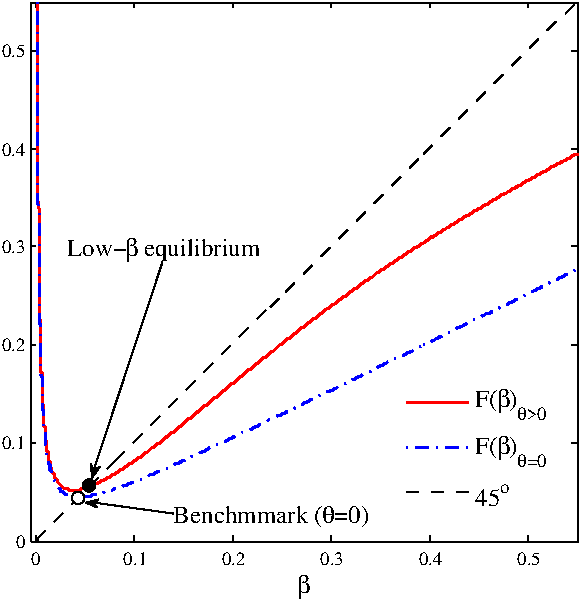
\includegraphics[width=67mm]{./Figures/fig_exogenous_low.pdf}
\label{low}}\quad
\subfigure [Large $\theta$ ($\theta=0.55$) $\Rightarrow$ unique high-$\beta$ equilibrium.]{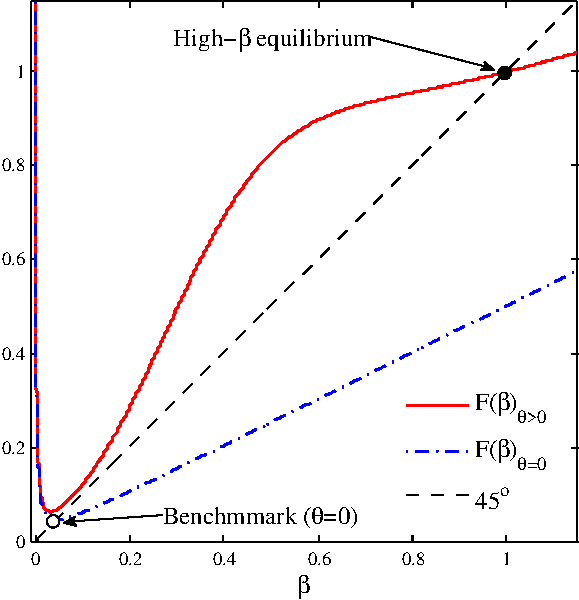
\includegraphics[width=67mm]{./Figures/fig_exogenous_high.pdf}\label{high}}\\[15pt]
\subfigure[Intermediate $\theta$ ($\theta=0.33$) $\Rightarrow$ multiple high-$\beta$ \& low-$\beta$ equilibria.]{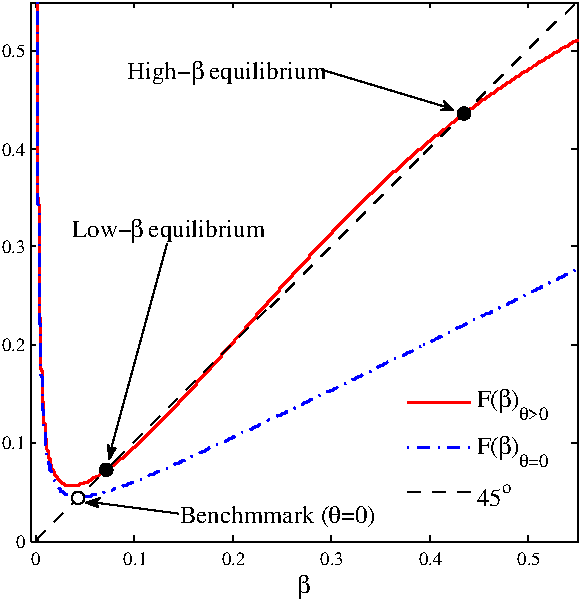
\includegraphics[width=67mm]{./Figures/fig_exogenous_multiple.pdf}\label{multi}}\\[10pt]
\caption{Determination of $\beta$}
\caption*{\footnotesize{Note: The figure plots $F(\beta)$ for different values of $\theta$. The equilibrium values of $\beta$ are determined at the fixed points of $F(\cdot)$.  The parameter values used in the figures are $\omega_{s}=50$, $\omega_{\delta}=1$, and $\omega_{u}=0.1$.}}
\label{fig:exog}
\end{figure}
